%-----------------------------------LICENSE------------------------------------%
%   This file is part of Mathematics-and-Physics.                              %
%                                                                              %
%   Mathematics-and-Physics is free software: you can redistribute it and/or   %
%   modify it under the terms of the GNU General Public License as             %
%   published by the Free Software Foundation, either version 3 of the         %
%   License, or (at your option) any later version.                            %
%                                                                              %
%   Mathematics-and-Physics is distributed in the hope that it will be useful, %
%   but WITHOUT ANY WARRANTY; without even the implied warranty of             %
%   MERCHANTABILITY or FITNESS FOR A PARTICULAR PURPOSE.  See the              %
%   GNU General Public License for more details.                               %
%                                                                              %
%   You should have received a copy of the GNU General Public License along    %
%   with Mathematics-and-Physics.  If not, see <https://www.gnu.org/licenses/>.%
%------------------------------------------------------------------------------%
\documentclass{article}
\usepackage{graphicx}                           % Needed for figures.
\usepackage{amssymb}                            % Needed for mathbb.
\usepackage{amsthm}                             % For the theorem environment.
\usepackage{amsmath}                            % Needed for align.
\usepackage[nottoc]{tocbibind}                  % Bibliography in toc.
\usepackage{xcolor}
\usepackage{listings}
\usepackage[font={scriptsize},
            hypcap=true,
            labelsep=colon]{caption}            % Figure captions.
\usepackage{hyperref}

\definecolor{background}{rgb}{0.9,0.9,0.9}

\lstdefinestyle{CStyle}{
    backgroundcolor=\color{background},
    commentstyle=\color{gray},
    keywordstyle=\color{blue},
    numberstyle=\tiny\color{red},
    stringstyle=\color{orange},
    basicstyle=\footnotesize,
    breakatwhitespace=false,
    breaklines=true,
    captionpos=b,
    keepspaces=true,
    numbers=left,
    numbersep=5pt,
    showspaces=false,
    showstringspaces=false,
    showtabs=false,
    tabsize=2,
    language=C
}

\hypersetup{
    colorlinks=true,
    linkcolor=blue
}

\theoremstyle{plain}
\newtheorem{theorem}{Theorem}

\title{An Iterative Algorithm for the Jones' Polynomial}
\author{Ryan Maguire\hspace{2em}Vladimir Chernov\hspace{2em}Peter Doyle}
\date{Fall 2021}

% No indent and no paragraph skip.
\setlength{\parindent}{0em}
\setlength{\parskip}{0em}

\begin{document}
    \maketitle
    \tableofcontents
    \begin{abstract}
        \noindent
        An iterative algorithm for computing the Jones' polynomial of a knot
        is described and an analysis of the computational complexity is given.
        A generalized conjecture about the Jones' polynomial is shown to be
        false via counterexample, and a conjecture generalizing Kronheimer and
        Mrowka's result on the unknot is made, with supporting numerical
        evidence.
    \end{abstract}
    \section{Extended Gauss Code}
        Given a knot diagram, it is reasonable for a mathematician to wish to
        describe the knot with finite data in such a way that a computer can
        understand and perform computations. This is achieved via Gauss code.
        Start by orienting the knot, labeling the crossings, and
        picking any point on the knot. You then walk along the knot, following
        the orientation, and keep track of the crossings you encounter. That is,
        we label the crossing number, and whether we're on the under strand or
        over strand with a $U$ or $O$, respectively. This is
        illustrated via example for the right-handed trefoil knot in
        Fig.~\ref{fig:right_handed_trefoil_gauss_code}.
        \begin{figure}
            \centering
            \includegraphics{../images/trefoil_knot_oriented_with_gauss_code.pdf}
            \caption{Gauss Code for the Right Handed Trefoil}
            \label{fig:right_handed_trefoil_gauss_code}
        \end{figure}
        Gauss code is not unique to a knot diagram since the code is dependent
        on the choice of starting point. This causes two different issues.
        First, when trying to determine if two knots are the same, we must
        check if one Gauss code is a cyclic permutation of another. Secondly,
        and more importantly, this version of Gauss code cannot distinguish
        between a knot and its mirror. If we take the left handed trefoil,
        give it a similar orientation as before, but choose a different
        starting point, we end up with
        Fig.~\ref{fig:left_handed_trefoil_gauss_code}. The resulting Gauss code
        is the same as the Gauss code we get for the right handed trefoil.
        The right handed and left handed trefoil knots are not equivalent
        (they have different Jones' polynomials), meaning Gauss code can't
        distinguish mirrors.
        \begin{figure}
            \centering
            \includegraphics{../images/trefoil_knot_mirror_oriented_with_gauss_code.pdf}
            \caption{Gauss Code for the Left Handed Trefoil}
            \label{fig:left_handed_trefoil_gauss_code}
        \end{figure}
        The solution is to \textit{sign} the crossings. Given an oriented knot,
        we label a crossing positive or negative depending on which strand is
        the over strand and which one is the under strand. This is shown in
        Fig.~\ref{fig:crossing_signs}.
        \begin{figure}
            \centering
            \includegraphics{../images/crossing_signs.pdf}
            \caption{Gauss Code for the Left Handed Trefoil}
            \label{fig:crossing_signs}
        \end{figure}
        By keeping track of the signs, in addition to whether or not we're on
        the under strand or over strand, we get the extended Gauss code. This
        is also called signed Gauss code.
        \begin{figure}
            \centering
            \includegraphics{../images/trefoil_knot_oriented_with_extended_gauss_code.pdf}
            \caption{Extended Gauss Code for the Right Handed Trefoil}
            \label{fig:right_hand_trefoil_extended_gauss}
        \end{figure}
        Note the orientation does not matter. If we reverse the orientation,
        the signs are still preserved. Examine Fig.~\ref{fig:crossing_signs} to
        convince yourself of this.
        \par\hfill\par
        Computationally, Extended Gauss code is a finite sequence of ordered
        triples. The length of the sequence is $2n$ where $n$ is the number of
        crossings in the diagram, and the ordered triples are of the form
        $(t,k,s)$ where $t\in\{O,U\}$, $s\in\{+1,-1\}$, and
        $0\leq{k}\leq{n-1}$ ($t$ for \textit{type}, $s$ for \textit{sign}, and
        $k$ for indexing). One could represent this in the C programming
        language as follows.
        \begin{lstlisting}[style=CStyle, gobble=12]
            enum crossing_sign {negative_crossing, positive_crossing};

            enum crossing_type {under_crossing, over_crossing};

            struct knot {
                unsigned int number_of_crossings;
                enum crossing_sign *sign;
                enum crossing_type *type;
                unsigned int *crossing_number;
            };
        \end{lstlisting}
        The pointers to the arrays \texttt{sign}, \texttt{type}, and
        \texttt{crossing\_number} each having 2 times
        \texttt{number\_of\_crossings} many elements.
        Similar definitions could easily be given with classes using the
        Python programming language. Regardless of preference, we now have a
        means of representing a knot in a computer.
        \par\hfill\par
        Not all finite sequences of length $2n$ will be valid Gauss code. For
        the code to be valid every integer $0\leq{k}\leq{n-1}$ must occur
        exactly twice, once with $t=O$ and once with $t=U$, and the sign
        $s$ must be the same for both crossings.
    \section{Virtual Knots}
        Consider the following Gauss code:
        \begin{equation}
            O0+O1+U0+U1+
        \end{equation}
        The code tells us we have a two crossing knot. A quick look through any
        table of knots tells us the smallest number of crossings a non-trivial
        knot can have is 3 (the left and right handed trefoils). The
        Reidemeister moves can translate to operations on extended Gauss code,
        but you'll find they're of no help here. Let's try to draw it
        (Fig.~\ref{fig:chain_link_fence_knot}).
        \begin{figure}
            \centering
            \includegraphics{../images/chain_link_fence_knot_virtual.pdf}
            \caption{The Chain Link Fence Knot}
            \label{fig:chain_link_fence_knot}
        \end{figure}
        To draw it on a piece of paper requires us to \textit{pretend} one of
        the crossing is fake, or \textit{virtual}. The problem of emedding
        graphs from graph theory tells us we really want to draw this on a
        higher genus surface.
        \begin{figure}
            \centering
            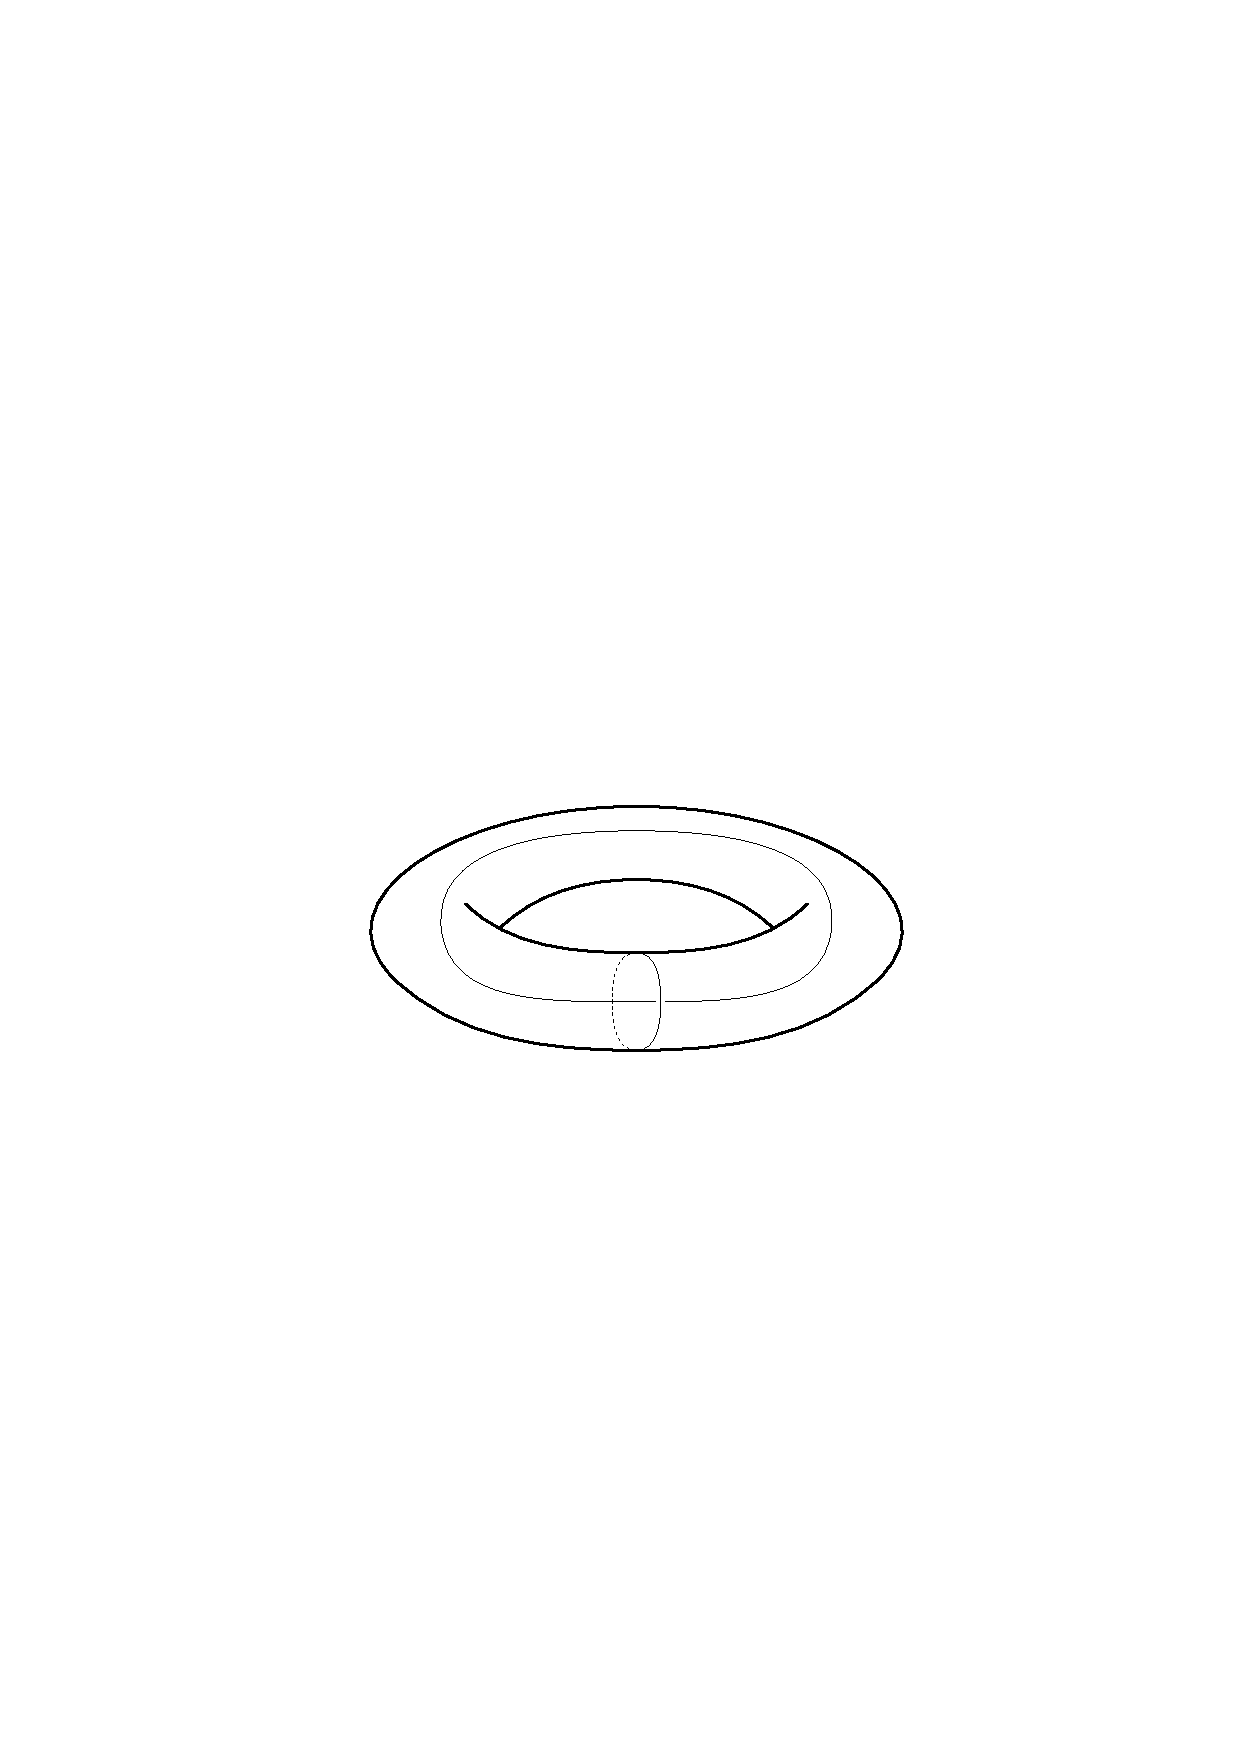
\includegraphics{../images/chain_link_fence_knot_on_torus.pdf}
            \caption{The Chain Link Fence Knot on a Torus}
            \label{fig:chain_link_fence_knot_on_torus}
        \end{figure}
        Using the torus $\mathbb{T}^{2}$ we can draw this knot without virtual
        crossings (Fig.~\ref{fig:chain_link_fence_knot_on_torus}).
        The label \textit{chain-link-fence} comes from trying to draw it
        on the flat torus
        (see Fig.~\ref{fig:chain_link_fence_knot_on_flat_torus}.)
        \begin{figure}
            \centering
            \includegraphics{../images/chain_link_fence_knot_on_flat_torus.pdf}
            \caption{The Chain Link Fence Knot on a Flat Torus}
            \label{fig:chain_link_fence_knot_on_flat_torus}
        \end{figure}
        Lifting this drawing to the universal cover, we see a chain-link fence
        (see Fig.~\ref{fig:chain_link_fence_knot_on_flat_torus_universal_cover}).
        These objects are called \textit{virtual knots}, knots that can be
        embedded into some 3-manifold of the form $M\times\mathbb{R}$ where
        $M$ is a smooth surface. A classical knot is just a virtual knot
        that can be embedded into $\mathbb{S}^{2}\times\mathbb{R}$.
        \begin{figure}
            \centering
            \resizebox{\textwidth}{!}{%
                \includegraphics{%
                    ../images/chain_link_fence_knot_on_flat_torus_universal_cover.pdf%
                }%
            }
            \caption{Lift of the Chain Link Fence Knot to $\mathbb{R}^{2}$}
            \label{fig:chain_link_fence_knot_on_flat_torus_universal_cover}
        \end{figure}
    \section{Resolving a Crossing}
        The Kauffman bracket polynomial is an invariant for
        \textit{framed links}. It is not a link invariant since the polynomial
        is not preserved by Reidemeister I moves (though this can be salvaged
        by a proper normalization, resulting in the Jones' polynomial). The
        definition we'll give in the next section is a mimicry of the
        description provided in \cite{barnatan2002khovanov}. It is recursive
        and requires us to \textit{resolve crossings}. Resolving a crossings
        equates to making it go away. There are two ways to do this.
        Given an unoriented knot diagram, we rotate our heads until
        the over crossing travels from the top left to the bottom right. The
        0 and 1 resolution of the crossing are given in
        Fig.~\ref{fig:resolving_crossing}.
        \begin{figure}
            \centering
            \includegraphics{../images/resolving_crossings.pdf}
            \caption{Resolving a Crossing}
            \label{fig:resolving_crossing}
        \end{figure}
        Given a knot diagram with $n$ crossings, and a number
        $0\leq{k}\leq{2}^{n}-1$, there is a unique resolution of all of the
        crossings corresponding to $k$. To obtain this we first label all of
        the crossings $0$ to $n-1$. Given a number $0\leq{k}\leq{2}^{n}-1$,
        we write $k$ in binary. The value of the $m^{th}$ bit in the
        binary representation of $k$ corresponds to how the $m^{th}$ crossing
        is smoothed. Take the left handed trefoil as an example with its
        standard knot diagram (Fig.~\ref{fig:left_handed_trefoil_gauss_code}).
        There are 3 crossings, so $2^{3}=8$ possible resolutions. The diagram
        in Fig.~\ref{fig:trefoil_knot_cube_of_resolutions} is called the
        \textit{cube of resolutions} for the left-handed
        trefoil. This language is slightly misleading since the cube of
        resolutions is dependent on the knot diagram, so it is better to say
        this is the cube of resolutions for the \textit{standard} diagram for
        the left-handed trefoil. The image gets complicated quickly since the
        size of the cube is exponential in the number of crossings. The cube of
        resolutions for the figure-eight knot is shown in
        Fig.~\ref{fig:figure_eight_knot_cube_of_resolutions}.
        \begin{figure}
            \centering
            \includegraphics{../images/trefoil_knot_cube_of_resolutions.pdf}
            \caption{Cube of Resolutions for the Left-Handed Trefoil}
            \label{fig:trefoil_knot_cube_of_resolutions}
        \end{figure}
        \begin{figure}
            \centering
            \resizebox{\textwidth}{!}{%
                \includegraphics{%
                    ../images/figure_eight_knot_cube_of_resolutions.pdf
                }
            }
            \caption{Cube of Resolutions for the Figure-Eight}
            \label{fig:figure_eight_knot_cube_of_resolutions}
        \end{figure}
        If we connect the appropriate images with arrows we would see a
        tesseract. The figure becomes messy with these arrows, and so have
        been omitted.
    \section{The Kauffman Bracket}
        The Kauffman bracket polynomial of a link $L$ is defined recursively
        in terms of smoothings of a link diagram. The definition is:
        \begin{align}
            \langle\emptyset\rangle&=1\\
            \langle{L\sqcup\mathbb{S}^{1}}\rangle&=(q+q^{-1})\langle{L}\rangle\\
            \langle{L}\rangle&=
                \langle{L_{m,0}}\rangle-q\langle{L_{m,1}}\rangle
        \end{align}
        where $L_{m,0}$ is the link obtained from the 0-smoothing of $L$ at
        the $m^{th}$ crossing, and $L_{m,1}$ is the link obtained from the
        1-smoothing at the $m^{th}$ crossing. The notation
        $\langle{L\sqcup\mathbb{S}^{1}}\rangle$ means the disjoint union of
        $L$ with an unknot. So, in particular, the Kaufmann bracket of the
        unknot is $q+q^{-1}$.
        \par\hfill\par
        The third equation reduces an $n$ crossing link to two $n-1$ crossing
        links. If we continue this recursive step we'll end up with
        $2^{n}$ completely resolved links, which is just the disjoint union of
        circles. Applying the second equation, we can inductively prove the
        following formula for the Kauffman bracket:
        \begin{equation}
            \langle{L}\rangle=\sum_{k=0}^{2^{n}-1}
                (-q)^{w(k)}(q+q^{-1})^{c(k)}
        \end{equation}
        Here, $w(k)$ is the Hamming weight of $k$. This is the number of 1's
        that occur in the binary expansion of $k$. Recalling that an integer
        $0\leq{k}\leq{2}^{n}-1$ represents a complete smoothing of a link,
        $c(k)$ is the number of circles that result from the $k$ smoothing.
        The Hamming weight is a well studied function in computer science and
        efficient methods of computing it are known. This includes
        constant-time algorithms if one restricts their attention to
        16-bit, 32-bit, or 64-bit unsigned integers, and the general algorithm
        can be done in $\log(k)$ time. To compute the Kauffman bracket, the
        only information needed is the number of circles that result from the
        $k^{th}$ smoothing ($0\leq{k}\leq{2}^{n}-1$). The point of this paper
        is to outline a simple algorithm that counts the number of circles in a
        smoothing using extended Gauss code. The code outlined works for knots,
        but simple extensions could be made for more general links. In
        particular, the algorithm works for \textit{virtual knots} and there is
        no restriction to the classical setting.
    \newpage
    \bibliographystyle{annotate}
    \bibliography{../biblio.bib}
    \newpage
    The source code used to generate this document is free software and released
    under version 3 of the GNU General Public License.
\end{document}
